We use the same event selections as in the SM Higgs search 
analysis~\cite{HWWHCP2012}. To improve the signal purity 
we use events in the 0-Jet bin and different flavor only. 
Two dimensional templates based on $m_T$ and $m_{\ell\ell}$ 
are used to extract the final search sensitivities as in the 
SM Higgs search analysis.
The templates are created with the following binnings,
%%%%%%%%%%%%%%%%%
\begin{itemize}
\item $m_T$ 14 bins: [60,70,80,90,100,110,120,140,160,180,200,220,240,260,280],
\item $m_{\ell\ell}$ bins: [12,30,45,60,75,100,125,150,175,200].
\end{itemize}
%%%%%%%%%%%%%%%%%
These binnings are chosen to ensure, 
%%%%%%%%%%%%%%%%%
\begin{itemize}
\item enough statistics for the main signal and background processes, 
\item enough granuarity in the signal enriched regions to distinguish between 
different hypotheses, 
\item the same binning in the background enriched (mainly $WW$ and $Top$) regions 
as in the SM Higgs analysis~\cite{HWWHCP2012}. 
\end{itemize}
%%%%%%%%%%%%%%%%%
Figure~\ref{fig:mtvsmll_sig} shows the $m_T-m_{\ell\ell}$ templates for the SM Higgs 
and the spin 2 graviton like resonances zoomed in the signal regions expected for \intlumiEightTeV, while 
Figure~\ref{fig:mtvsmll_bkg} shows the corresponding background templates. 

For a given dataset we construct two different models based on the $m_T-m_{\ell\ell}$ 
templates for the two different signal hypotheses, applying the 
same event selections and background predictions are used.  
In each model the specific signal templates are used with the 
signal strength left float in the CLs fit. 
The difference in the best fit likelihoods is then used 
to quantify the consistency between data and each signal hypothesis. 
In calculating the expected separation between the SM Higgs and other 
exotic resonances, we use the same number of events after the full selections as in 
the SM Higgs case. 

%%%%%%%%%%%%%%%%%%%%%%%%%%%%%%%%%%%%%%%%%%%%%
\begin{figure}[!hbtp]
\centering
\subfigure[SM Higgs]{
\centering
\label{subfig:hww}
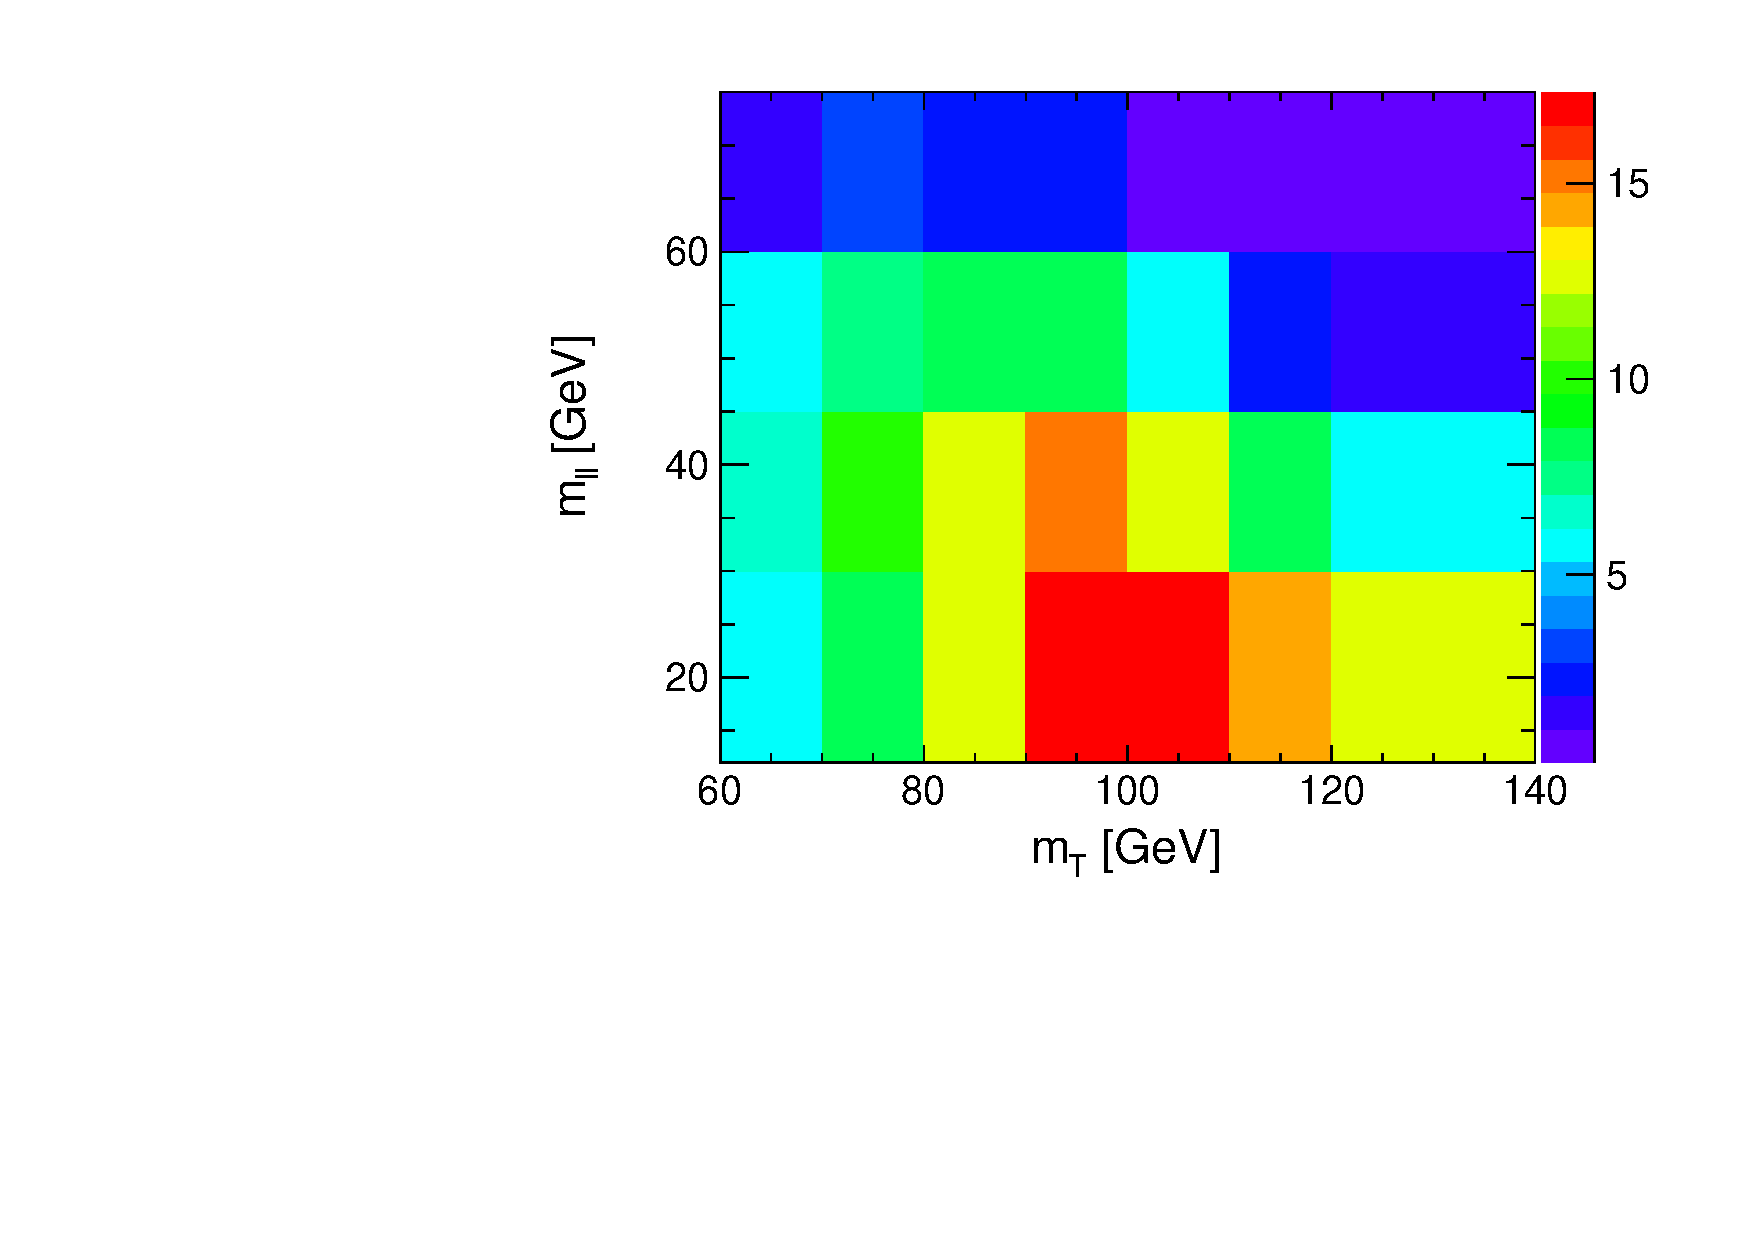
\includegraphics[width=.45\textwidth]{figures/mtvsmll_hww.pdf}
}
\subfigure[Graviton ($2_m^+$)]{
\centering
\label{subfig:xww}
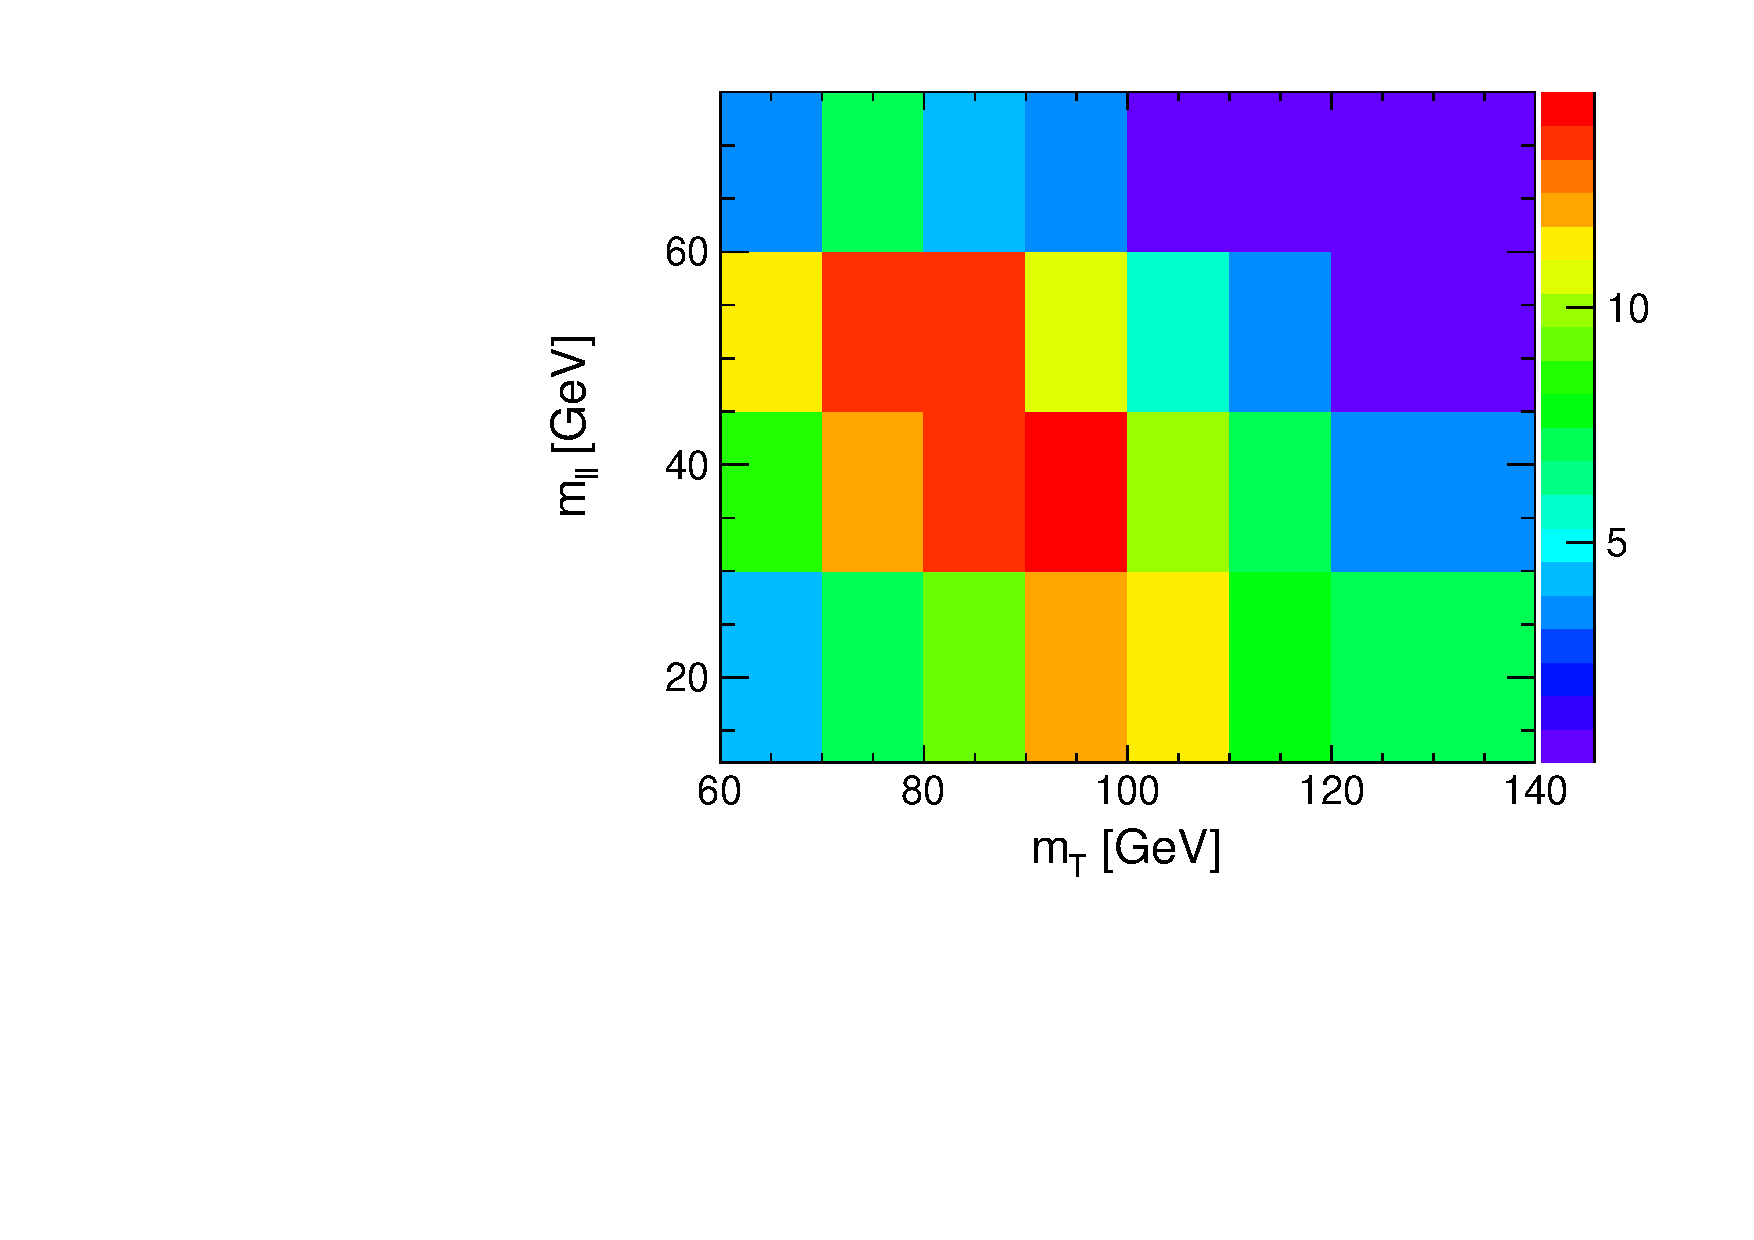
\includegraphics[width=.45\textwidth]{figures/mtvsmll_xww.pdf}
}\\
\caption{The $m_T-m_{\ell\ell}$ templates for the SM Higgs and 
spin 2 graviton like resonances, zoomed in 
the signal regions. The distributions are 
normalized to the expectations for \intlumiEightTeV.}
\label{fig:mtvsmll_sig}
\end{figure}
%%%%%%%%%%%%%%%%%%%%%%%%%%%%%%%%%%%%%%%%%%%%%


%%%%%%%%%%%%%%%%%%%%%%%%%%%%%%%%%%%%%%%%%%%%%
\begin{figure}[!hbtp]
\centering
\subfigure[$qq\to WW$]{
\centering
\label{subfig:qqww}
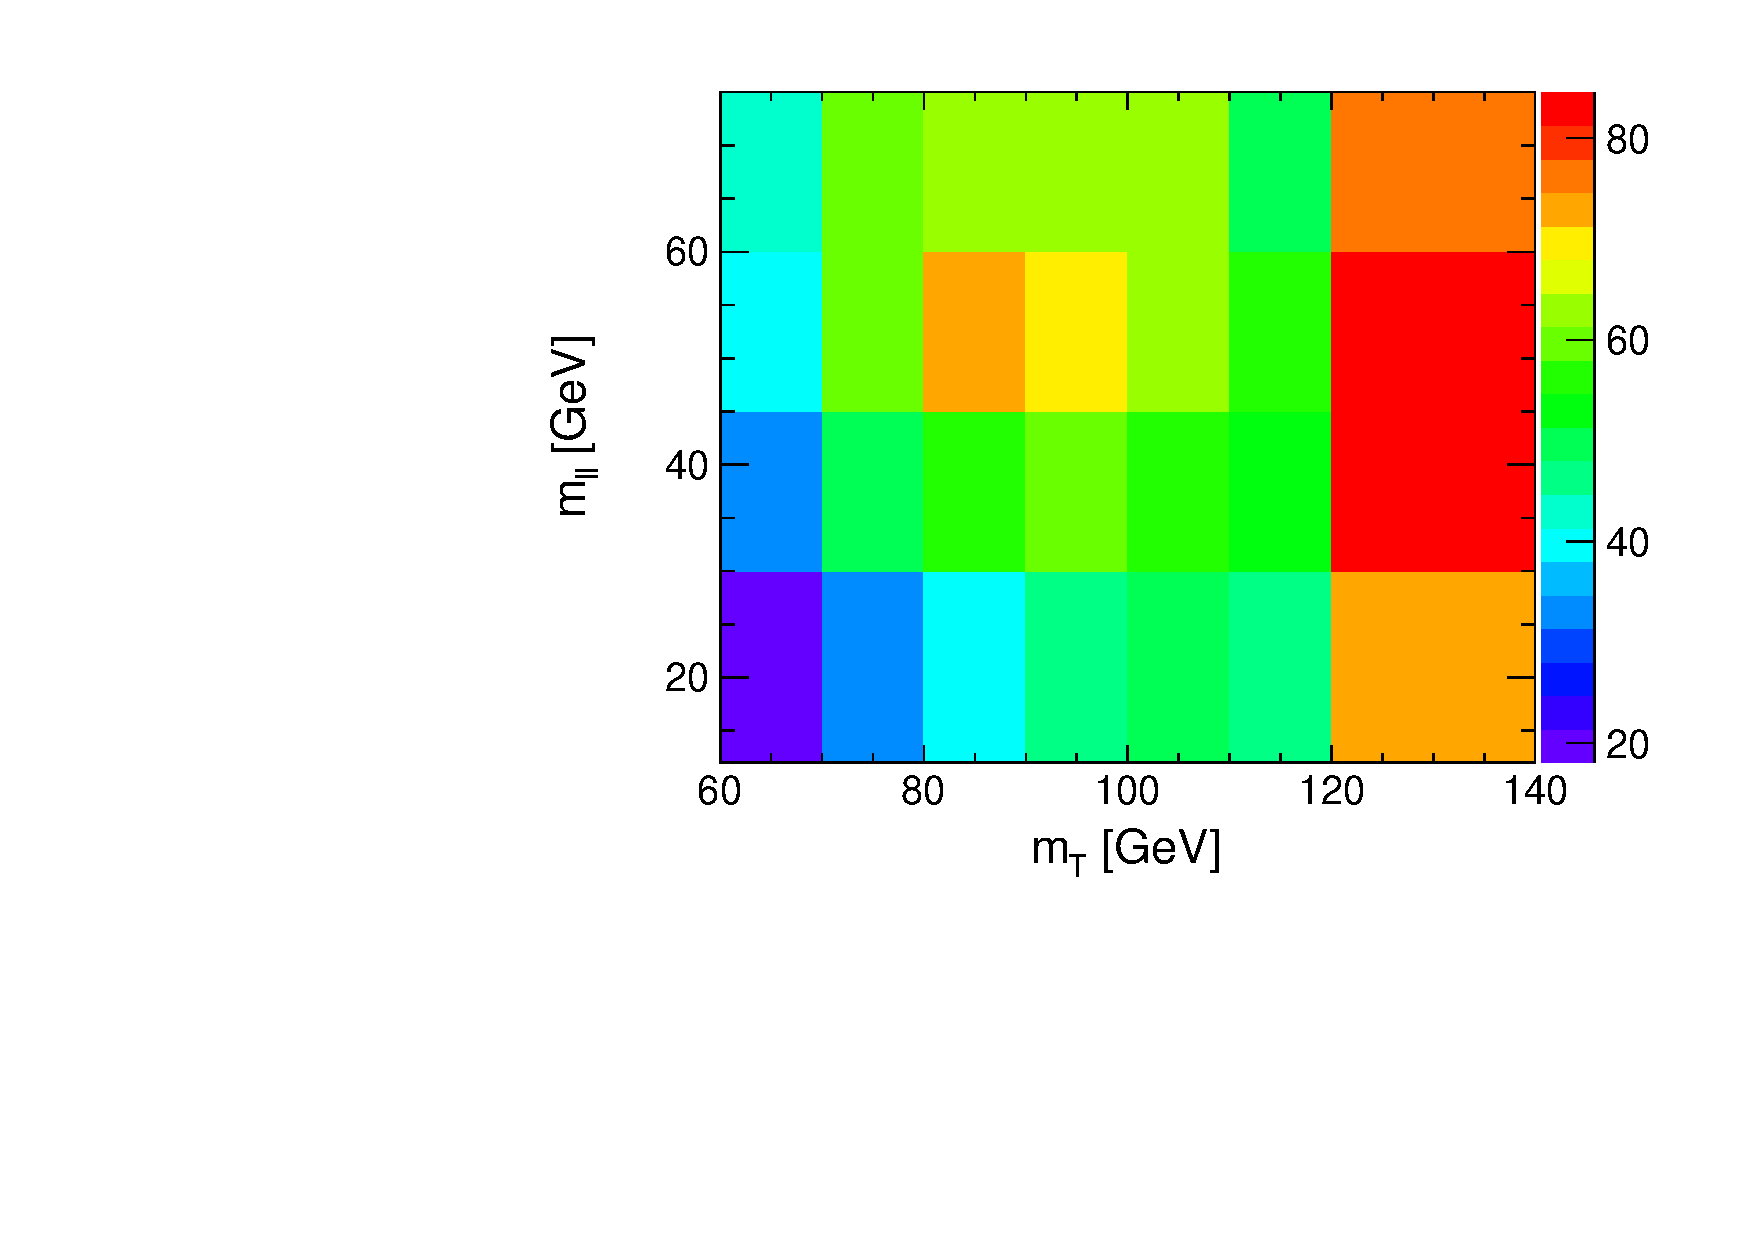
\includegraphics[width=.45\textwidth]{figures/mtvsmll_qqWW.pdf}
}
\subfigure[W+Jets]{
\centering
\label{subfig:wjets}
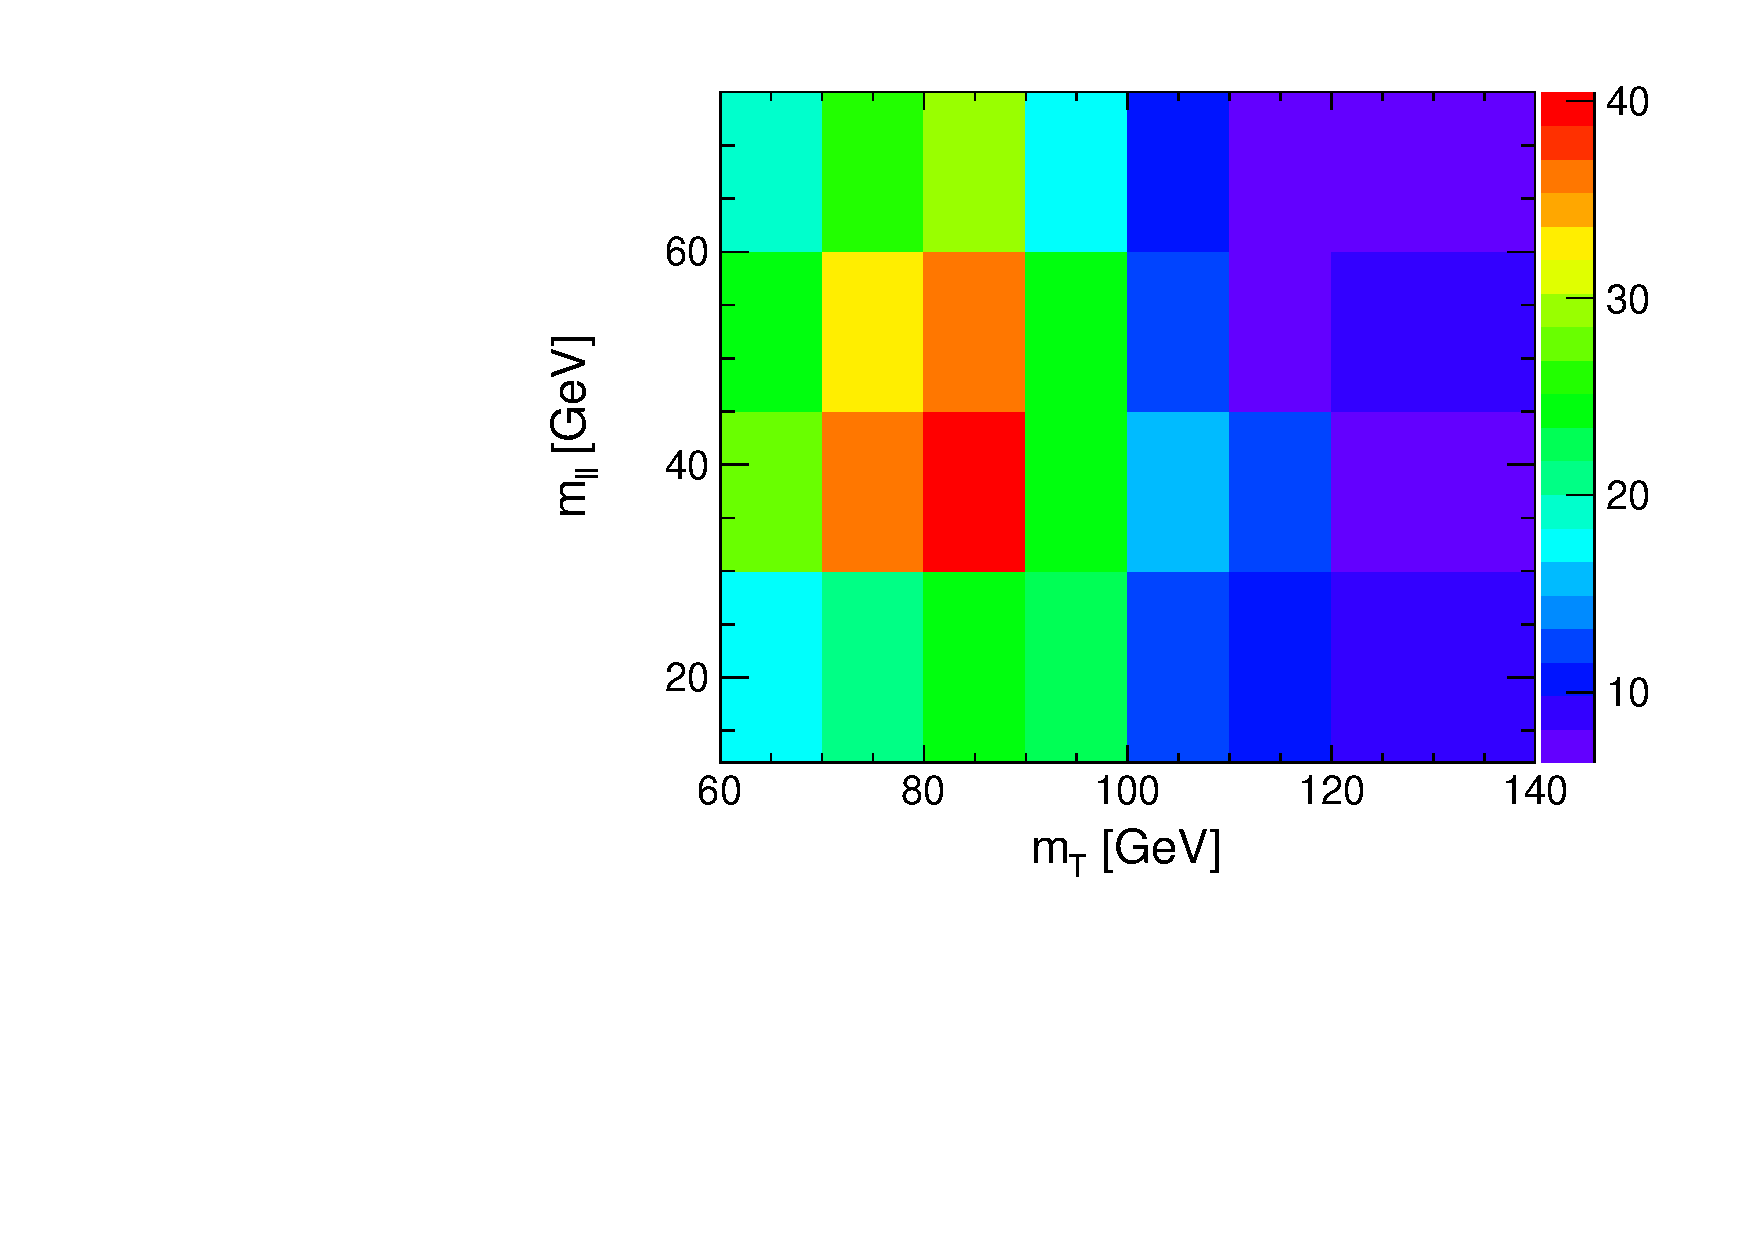
\includegraphics[width=.45\textwidth]{figures/mtvsmll_Wjets.pdf}
}\\
\subfigure[$W\gamma$]{
\centering
\label{subfig:wgamma}
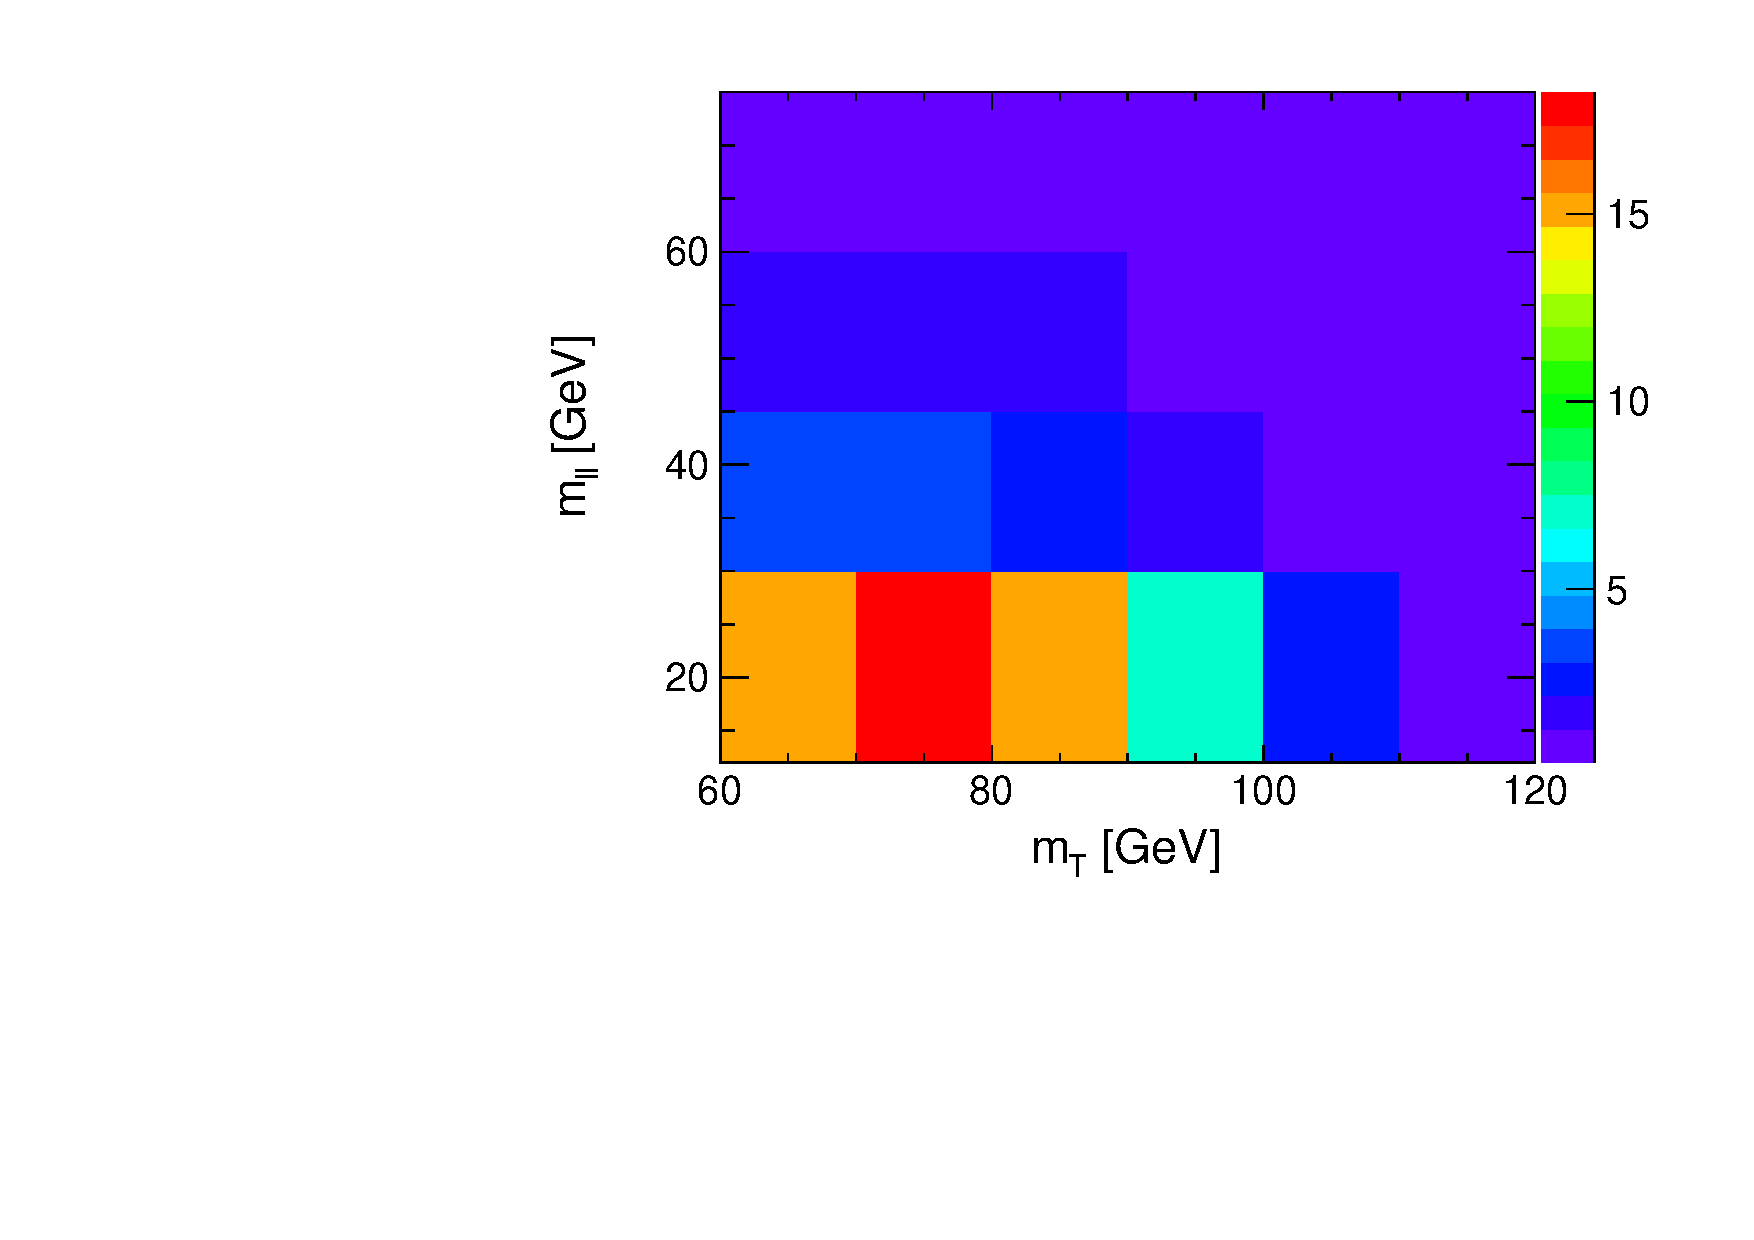
\includegraphics[width=.45\textwidth]{figures/mtvsmll_Wgamma.pdf}
}
\subfigure[$W\gamma^*$]{
\centering
\label{subfig:wgst}
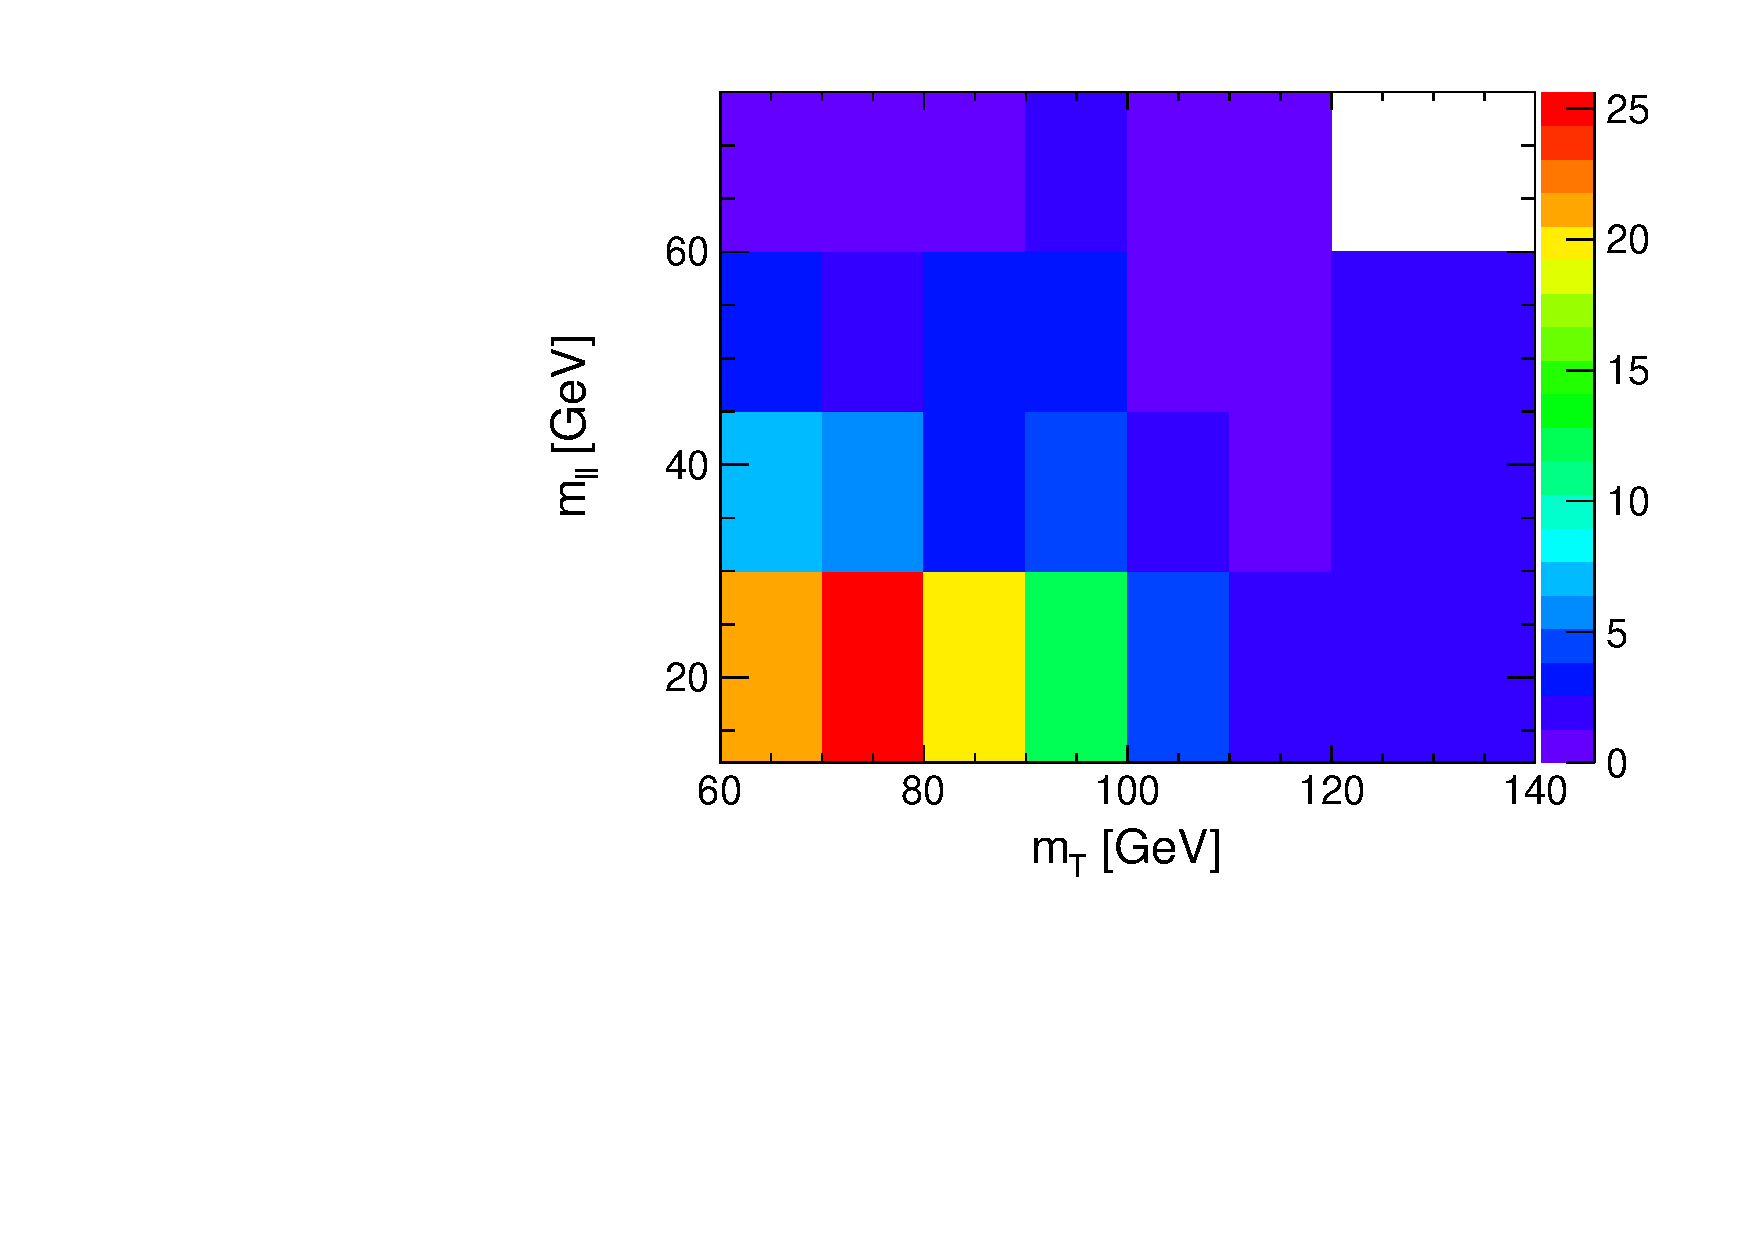
\includegraphics[width=.45\textwidth]{figures/mtvsmll_Wgstar.pdf}
}\\
\subfigure[Top]{
\centering
\label{subfig:top}
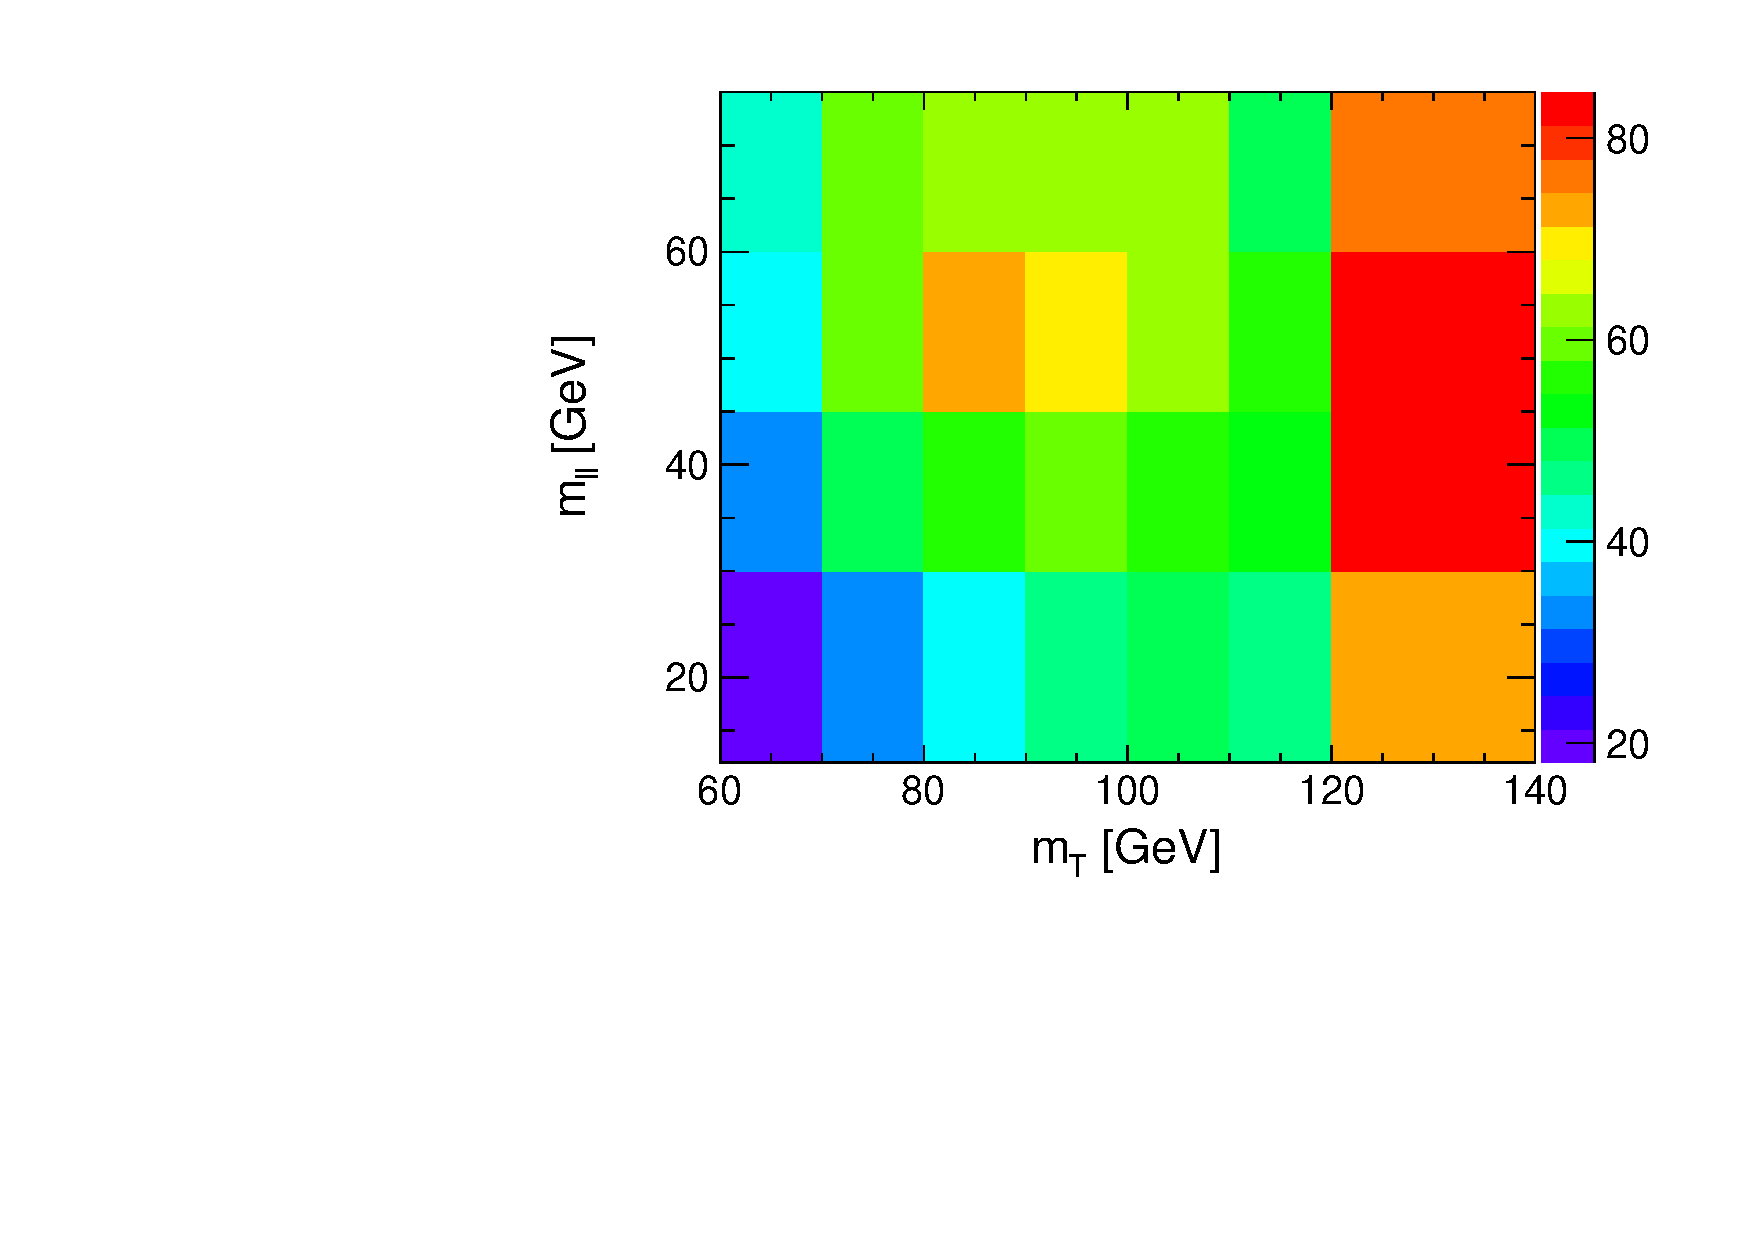
\includegraphics[width=.45\textwidth]{figures/mtvsmll_qqWW.pdf}
}
\subfigure[VV]{
\centering
\label{subfig:vv}
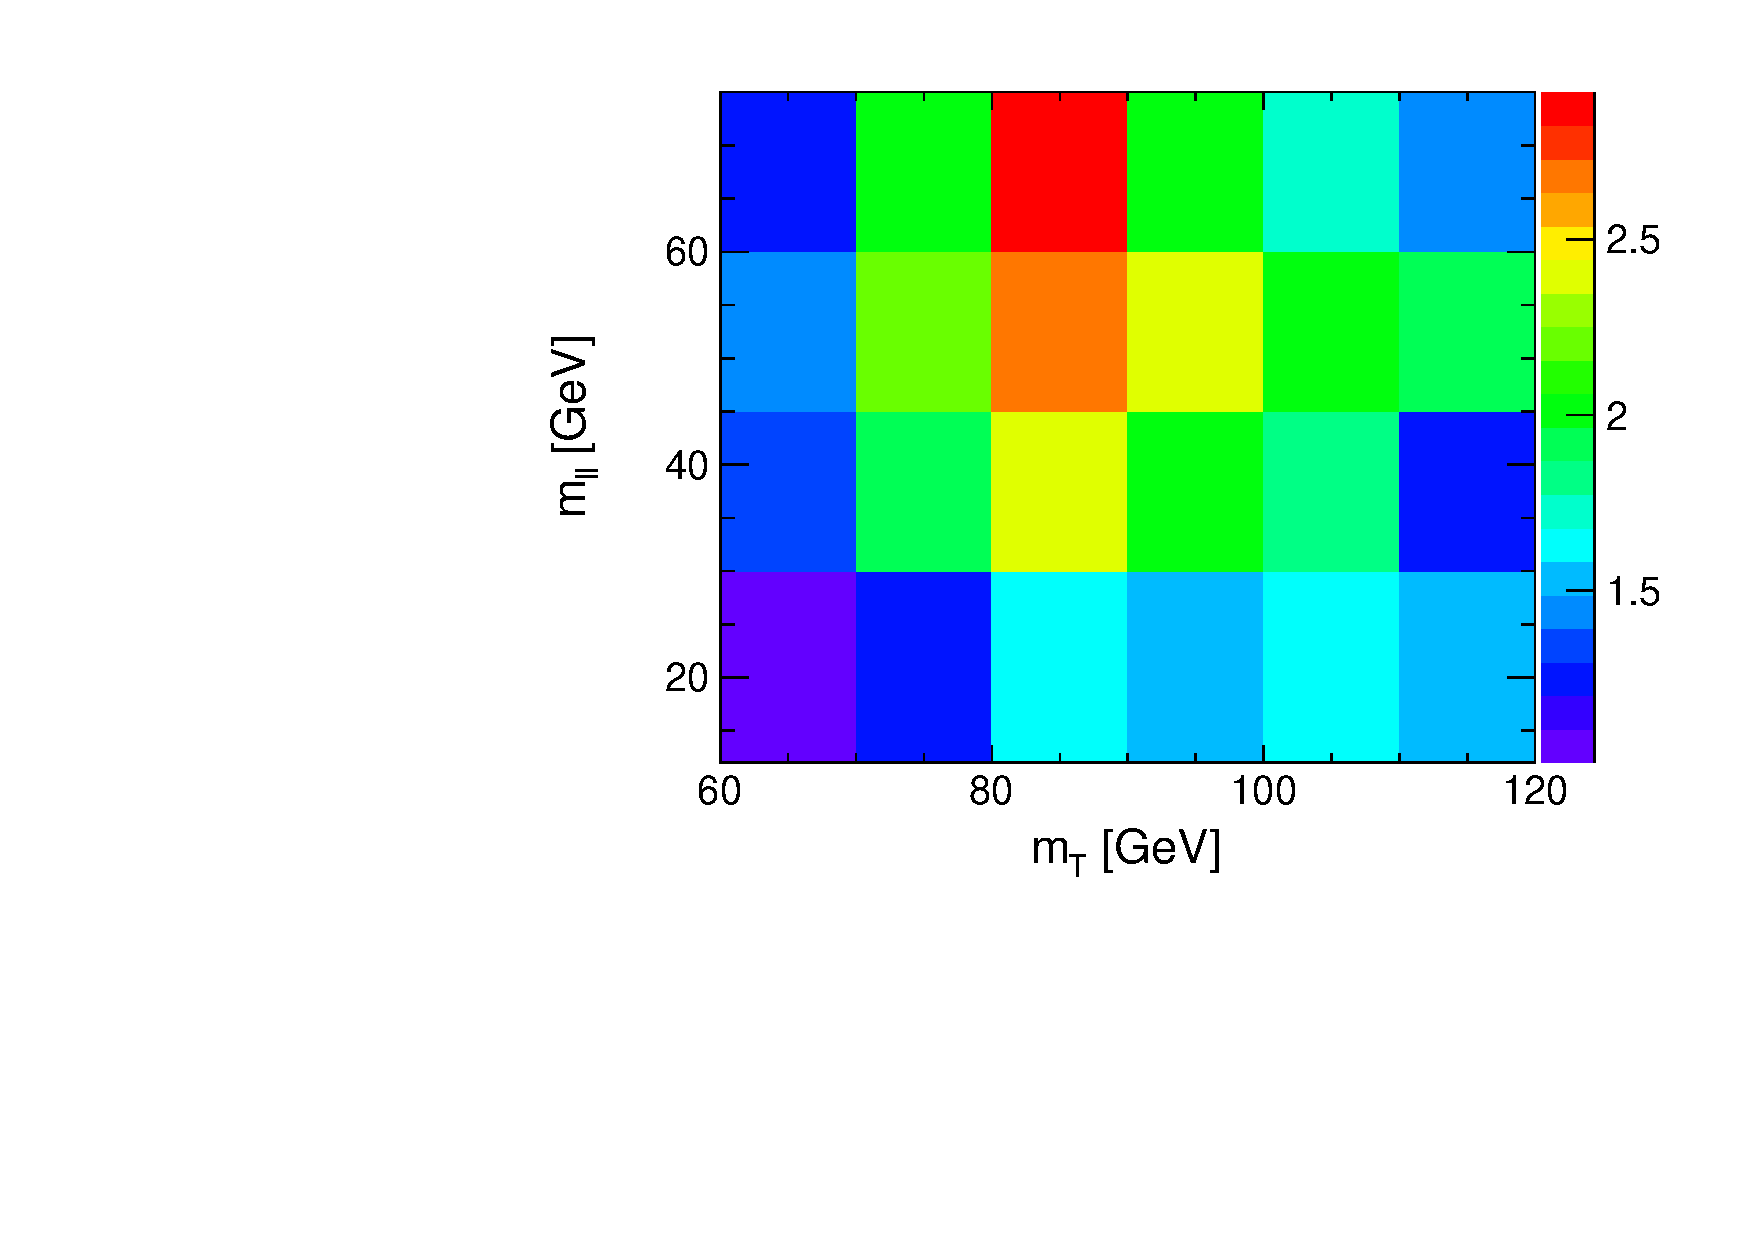
\includegraphics[width=.45\textwidth]{figures/mtvsmll_VV.pdf}
}\\

\caption{The $m_T-m_{\ell\ell}$ templates for the backgrounds, zoomed in 
the signal regions. The distributions are 
normalized to the expectations for \intlumiEightTeV.}
\label{fig:mtvsmll_bkg}
\end{figure}
%%%%%%%%%%%%%%%%%%%%%%%%%%%%%%%%%%%%%%%%%%%%%